\chapter{Introduction}
% The goal of this chapter is to give an overview of the available knowledge about stearoyl-CoA desaturase (SCD1) which is the main focus of this thesis. SCD1 is an iron-containing enzyme and member of the large non-heme iron enzyme family. The chapter starts  explaining the role of iron in biological systems and moves on to discuss the experimental and theoretical methods used to study non-heme iron enzymes. An overview of the rich chemistry of both binuclear and mononuclear non-heme iron enzymes is given before discussing the reactivity and importance of SCD1.

\section{Role of phosphates in biological systems}
Phosphates are one of the building blocks that play central role to the life on our planet Earth. They form the basis for both the storage and transfer of genetic information and the flow of metabolic energy within biological systems. The ubiquitous nature of phosphate esters and anhydrides, such as those found in deoxyribonucleic acid (DNA), ribonucleic acid (RNA), adenosine triphosphate (ATP), as well as polyphosphate (polyP) highlights their fundamental importance \citep{westheimerWhyNatureChose1987}. Some of the phosphates found in biological systems and their respective functions can be found in Table~\ref{tab:role_of_phosphates}.

A key characteristic enabling these roles is the ability of phosphoric acid to link molecular units whilst retaining an ionisable group. This inherent negative charge at physiological pH serves a dual purpose: it helps preserve these molecules within cellular boundaries defined by lipid membranes, and more importantly, it gives kinetic stability upon phosphate esters and anhydrides by electrostatically repelling nucleophilic attack, particularly from water \citep{westheimerWhyNatureChose1987}. For instance, the half-time of hydrolysis at 25\textdegree C for phosphomonoester monoanion (P-O) is about 90 years, however for phosphodiester anion (P-O) this number rockets all the way to 16 million years \citep{wolfendenDegreesDifficultyWaterConsuming2006}. This  stability is of great importance when it comes to the integrity of genetic material but is easily overcome by enzymatic catalysis when there is a metabolic demand.

Phosphates are involved in numerous processes in living systems, e.g. cell signalling and sensation, metabolism regulation, blood coagulation, and bone formation \citep{mullerInorganicPolyphosphatesStorage2019, nebesnayaInorganicPolyphosphateRegulates2024}. The role of phosphates is perhaps most evident in cellular energetics, where ATP serves as the universal energy currency. The energy derived from the nutrients like glucose is captured and stored within the high-energy phosphoanhydride bonds linking the phosphate groups of ATP. This energy is released upon the hydrolysis of the terminal phosphoanhydride bond, typically yielding adenosine diphosphate (ADP) and inorganic phosphate (P\textsubscript{i}). The bond cleavage in this case provides the thermodynamic driving force for the majority of cellular processes, including biosynthesis, active transport, and mechanical work like muscle contraction. The standard free energy change for ATP hydrolysis is substantial ($\Delta G^{0}=-30.5$ kJ mol$^{-1}$), and under cellular conditions, the actual free energy release is often considerably greater. To be specific, the experimentally obtained $\Delta G$ values in liver are about $-59$ to $-53.5$ kJ mol$^{-1}$, and in the heart about $-61.7$ to $-59.5$ kJ mol$^{-1}$ \citep{mullerInorganicPolyphosphatesStorage2019}.

\begin{table}[b!]
    \centering
    \begin{tabular}{cc}
    \toprule
    \textbf{Phosphate} & \textbf{Biological role} \\ 
    \midrule
    DNA/RNA & Genetic material \\
    ADP/ATP & Intracellular energy transfer \\
    cAMP & Cellular signalling \\
    Polyphosphate & Energy storage, Cellular signalling \\
    Creatine phosphate & Intracellular energy transfer \\
    Phosphoenolpyruvate & Metabolism \\
    Pyridoxal phosphate & Coenzyme \\
    Nicotine adenine dinucleotide & Calcium signaling \\
    Fructose 1,6-diphosphate & Metabolism \\
    Glucose-6-phosphate & Metabolism \\
    Isopentenyl pyrophosphate & Metabolism \\
    Ribose-6-phosphate & Metabolism \\
    Glycerol 3-phosphate & Metabolism \\
    Dihydroxyacetone phosphate & Calvin cycle, metabolism \\
    Inositol phosphates & Cellular signaling \\
    \bottomrule
    \end{tabular}
    \caption{Examples of biologically relevant phosphates and their roles. Reproduced and adapted from~\citep{kamerlinWhyNatureReally2013}.}
    \label{tab:role_of_phosphates}
\end{table}

Beyond ATP, inorganic polyphosphate (polyP), a linear polymer of orthophosphate residues linked by similar high-energy phosphoanhydride bonds, represents another significant phosphate-based energy store found across all domains of life, including mammalian cells, even though in mammalian cells the concentration of polyP is significantly lower comparing to microorganisms. While its roles in mammals are still being fully elucidated, polyP metabolism is intrinsically linked to cellular energy status. Mitochondrial polyP levels fluctuate with respiratory activity and appear dependent on F\textsubscript{0}F\textsubscript{1}-ATP synthase function, suggesting a role in mitochondrial bioenergetics, potentially acting as an energy reservoir \citep{pavlovInorganicPolyphosphateEnergy2010}.

The efficient transfer of energy stored in phosphate bonds from sites of production (e.g., mitochondria) to sites of utilisation (e.g., ATPases involved in muscle contraction or ion transport) is crucial. Simple diffusion of ATP is often insufficient due to intracellular structure and the potential for large concentration gradients to develop, which would be thermodynamically inefficient. Instead, cells employ phosphotransfer networks, utilising enzymes like creatine kinase and adenylate kinase that catalyse rapid, near-equilibrium phosphoryl exchange reactions. These networks act as 'phosphoryl wires', facilitating the efficient conduction of high-energy phosphoryl groups and energetic signals throughout the cell with minimal dissipation of energy or accumulation of inhibitory products like ADP. The existence of these networks underscores the dynamic and highly organised nature of cellular energy management, where phosphates, primarily in the form of ATP, act as the key energy carriers \citep{dzejaPhosphotransferNetworksCellular2003}.

The synthesis of ATP primarily occurs through oxidative phosphorylation in mitochondria, a process tightly coupled to the electron transport chain which establishes a proton-motive force (PMF) across the inner mitochondrial membrane. This electrochemical potential energy is harnessed by the remarkable molecular machine, ATP synthase. Interestingly, the principal energy input required by ATP synthase is not for the chemical formation of the phosphoanhydride bond itself, but rather for the conformational changes needed to release the newly synthesised, tightly bound ATP molecule from the enzyme's catalytic site. This 'binding change mechanism' involves cooperative, sequential action of the enzyme's multiple catalytic sites, driven by proton flow. The hydrolysis of ATP to ADP and Pi is catalysed by a variety of enzymes, including ATPases and potentially F\textsubscript{1}-ATPase, which are often coupled to other cellular processes \citep{boyerEnergyLifeATP1998}.

In essence, the unique chemical properties of phosphates - their ability to form stable esters and energy-rich anhydrides that have negative charge - coupled with the evolution of sophisticated enzymatic machinery for their synthesis, transfer, and hydrolysis have secured their vital role in virtually all life processes.


\section{Enzymes involved in phosphate hydrolysis}



\section{Reaction mechanism}

\begin{figure}[htbp]
    \centering
    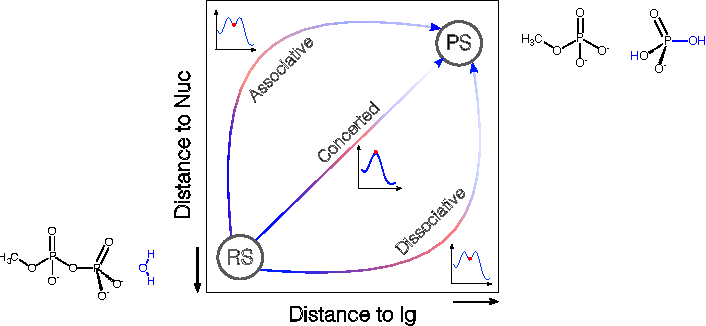
\includegraphics[width=0.5\textwidth]{Figures/1_Introduction/intro_mfj_plot.pdf}
    \caption{MFJ plot.}
    \label{fig:mfj_plot}
\end{figure}

\subsection{S\textsubscript{N}1 and S\textsubscript{N}2 nucleophilic substitution reactions}

\begin{figure}[htbp]
    \centering
    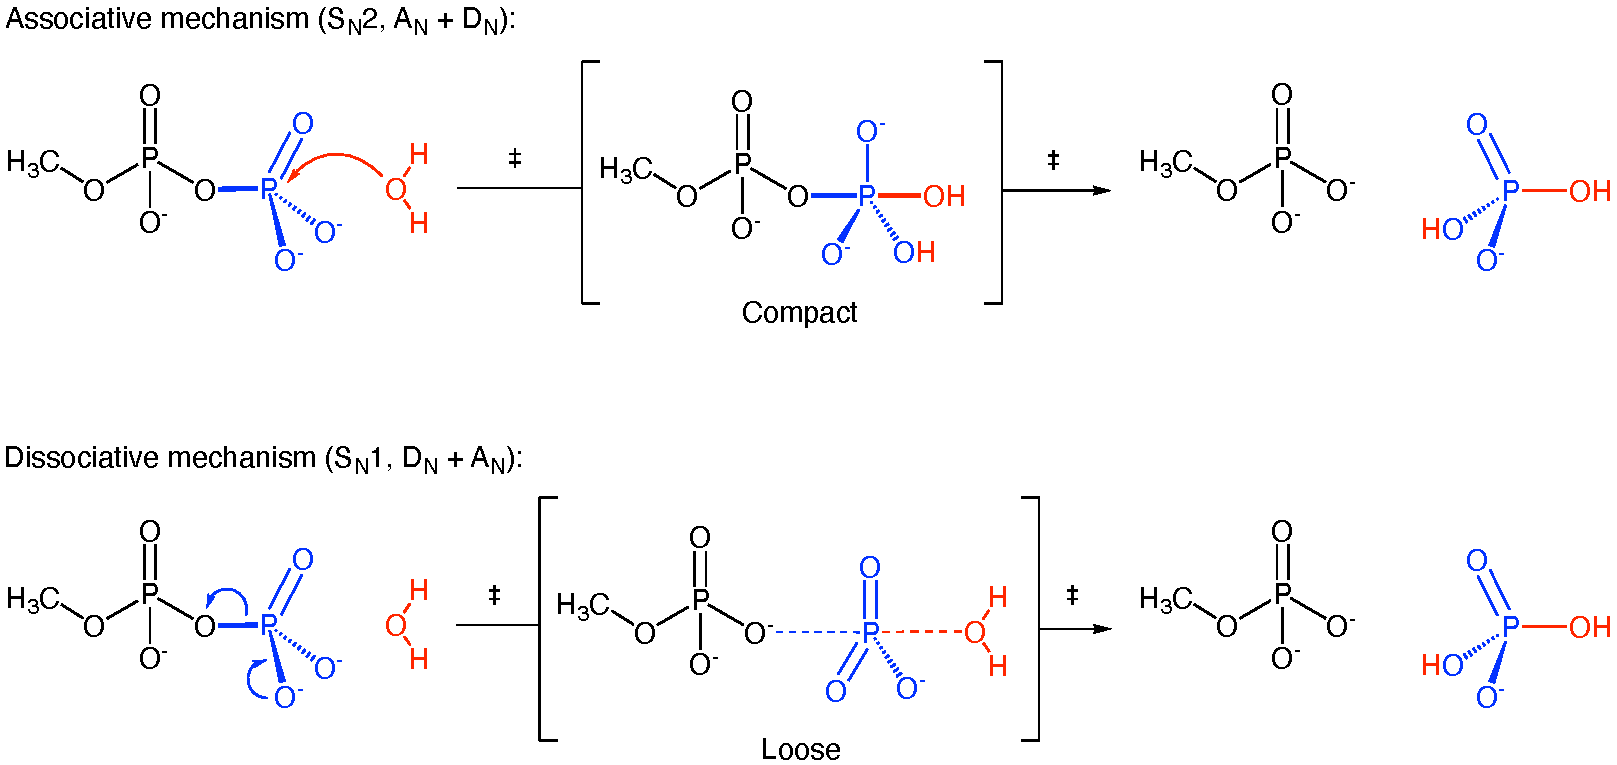
\includegraphics[width=0.95\textwidth]{Figures/1_Introduction/intro_reaction_mechanism.pdf}
    \caption{Reaction mechanism.}
    \label{fig:reaction-mechanism}
\end{figure}


\section{Research goals}


